\documentclass[11pt]{article}
\usepackage[margin=1in]{geometry}
\usepackage{amsmath,amssymb}
\usepackage{graphicx}
\usepackage{booktabs}
\usepackage{hyperref}
\usepackage{xcolor}

\title{The Birth Bias Axis: Probing the Allen-Cahn--Burgers Universality
       Class Transition in VCML}
\author{Gabriel Aubin-Moreau}
\date{2026}

\begin{document}
\maketitle

\begin{abstract}
Papers~22 and~23 established that within-zone spatial correlations in VCML
obey Allen-Cahn interface sharpening dynamics: the correlation length $\xi$
\emph{decreases} over time (exponent $\beta < 0$), and $\xi_\infty$ is set
by the balance of site-level diffusion $\kappa$ and the consolidation-driven
restoring force.
In Allen-Cahn dynamics, the birth rule selects a \emph{uniform-random} neighbour,
creating symmetric diffusion with no net advection.
Here we test whether replacing this rule with \emph{fitness-proportionate}
selection (newborns preferentially inherit from the highest-$|F|$ neighbour)
injects an advection term $u\,\partial F/\partial x$ into the effective PDE
and shifts the system toward the Burgers/Fisher-KPP universality class
($\xi$ increasing, $\beta > 0$).
We sweep the birth bias $\alpha \in \{0.0, 0.2, 0.4, 0.6, 0.8, 1.0\}$,
where $\alpha=0$ recovers current VCML (Allen-Cahn) and $\alpha=1$ is
fully fitness-proportionate (Burgers candidate).
The predicted sign flip in $\Delta\xi = \xi_{\rm late} - \xi_{\rm early}$
is \emph{not} observed: all values of $\Delta\xi$ remain negative across
the full $\alpha$ range.
However, $\xi_{\rm late}$ increases monotonically from $2.4$ to $4.6$ sites
as $\alpha$ goes from $0$ to $1$, and zone differentiation sg4 is enhanced
at $\alpha=1.0$.
We attribute the absence of the full Burgers transition to the
$\nu/\kappa = 0.001/0.020 = 0.05 \ll 1$ regime: at standard parameters,
the advection term (strength $\propto \nu$) is approximately $20\times$
weaker than the diffusion term (strength $\propto \kappa$), insufficient
to overcome the restoring force that pins the system in the Allen-Cahn
basin.
The birth bias axis is identified as the control parameter for the
Allen-Cahn--Burgers transition in VCML, and the critical $\nu/\kappa$ ratio
for the transition is estimated to be $\sim 1$.
\end{abstract}

%----------------------------------------------------------------------
\section{Introduction}
%----------------------------------------------------------------------

Paper~22 discovered that VCML zone formation is an instance of Allen-Cahn
phase separation: the within-zone spatial correlation length $\xi(t)$
\emph{decreases} during zone formation, from ${\sim}20$ sites (early,
when $F \approx 0$) to $\xi_\infty \approx 2$--$4$ sites (equilibrium).
Paper~23 confirmed that $\xi_\infty = C_{\rm geo}\,\sqrt{\kappa/(P_c \cdot FA)}$
and identified two effective PDEs governing the system through a
Reynolds decomposition $F = \bar{F}_z + F_{\rm res}$:

\begin{align}
  \text{(PDE 1, zone-mean):}\quad
  \tau_{\rm base}\,\partial_t \bar{F}_z &= P_c\cdot FA\cdot(\bar{m}_z - \bar{F}_z) \label{eq:pde1} \\
  \text{(PDE 2, within-zone):}\quad
  \partial_t F_{\rm res} &= \kappa\,\nabla^2 F_{\rm res}
                            + P_c\cdot FA\cdot(m_{\rm res} - F_{\rm res}). \label{eq:pde2}
\end{align}

PDE~2 is Allen-Cahn with diffusivity $\kappa$ and restoring-force constant
$P_c \cdot FA$.
The Allen-Cahn classification requires symmetric diffusion, which arises
because the birth rule selects a \emph{uniform-random} neighbour: no
directional bias means no net advection.

The natural question is: what happens if we break this symmetry?
If newborns preferentially copy from the \emph{highest-$|F|$} neighbour,
the copy step introduces a directional bias proportional to the local
$|F|$ gradient, which enters the effective PDE as an advection term.
Schematically:
\begin{equation}
  \partial_t F = \kappa\,\nabla^2 F + \underbrace{\nu\,u(F)\,\nabla F}_{\rm advection}
                 + P_c\cdot FA\cdot(m - F),
  \label{eq:pde_full}
\end{equation}
where $u(F)$ is an effective velocity field proportional to the local
$|F|$ amplitude and $\nu$ is the turnover rate controlling how often
births inject the advection signal.
When the advection term dominates ($\nu \gg \kappa$), the system enters
the Burgers/Fisher-KPP universality class where $\xi$ grows rather than
shrinks.
The Model~H framework (Hohenberg and Halperin, 1977) contains both
limits: Allen-Cahn ($u = 0$) and Navier-Stokes/Burgers ($\xi \to \infty$).

We test this prediction by introducing a continuous birth bias parameter
$\alpha \in [0,1]$ that interpolates between uniform random selection
($\alpha=0$, Allen-Cahn) and fully fitness-proportionate selection
($\alpha=1$, Burgers candidate).

%----------------------------------------------------------------------
\section{Methods}
%----------------------------------------------------------------------

\paragraph{Birth bias implementation.}
At each death event, the newborn's $F$ seed is drawn from a neighbour $j$:
\begin{itemize}
  \item With probability $1-\alpha$: $j$ is chosen uniformly at random
        from neighbours (current VCML rule).
  \item With probability $\alpha$: $j = \arg\max_{k \in \mathcal{N}}|F_k|^2$
        (fitness-proportionate, preferring high-amplitude neighbours).
\end{itemize}
In the fitness-proportionate branch, if multiple neighbours have equal
$|F|^2$, the selection is proportional to $|F_k|^2$ (softmax with
identity temperature).

\paragraph{Sweep.}
$\alpha \in \{0.0, 0.2, 0.4, 0.6, 0.8, 1.0\}$, five seeds each (30 runs total).
Standard parameters: $\nu=0.001$, $FA=0.40$, $\kappa=0.020$, $T_{\rm end}=3000$,
checkpoints every 200 steps.
Grid: $H=20$, $\mathrm{HALF}=20$, $N_{\rm zones}=4$, zone width 5 sites.

\paragraph{Measurements.}
At each checkpoint:
\begin{itemize}
  \item sg4: mean pairwise L2 distance between zone-mean $F$ vectors.
  \item $C(r)$ with zone-mean subtraction: within-zone autocorrelation
        (as in Paper~22), used to extract $\xi(t)$.
  \item $C_{\rm full}(r)$ without subtraction: zone-level autocorrelation.
\end{itemize}
$\xi$ is extracted via log-linear regression $C(r) = e^{-r/\xi}$ for
$r=1\ldots\min(5, 10)$, with $\xi > 30$ excluded as outliers.

%----------------------------------------------------------------------
\section{Results}
%----------------------------------------------------------------------

\subsection{All $\xi(t)$ trajectories decrease: Allen-Cahn persists}

Figure~1A shows the mean $\xi(t)$ trajectory for all six $\alpha$ values.
Every trajectory exhibits the same qualitative pattern: $\xi$ starts
large (${\sim}20$--$30$ sites at early times, when $F \approx 0$) and
decreases to a small equilibrium value by $t \approx 2000$.
This is the Allen-Cahn interface-sharpening signature established in
Paper~22, and it persists across the full $\alpha$ range.
The Burgers prediction of a \emph{growing} $\xi$ is not observed for any
value of $\alpha$.

\subsection{$\xi_{\rm late}$ increases monotonically with $\alpha$}

Although the qualitative trajectory does not change, the \emph{equilibrium
level} $\xi_{\rm late}$ (mean over $t \geq 2400$) does show a clear and
monotone increase with $\alpha$ (Figure~1B, Table~\ref{tab:results}).
From $\alpha=0$ to $\alpha=1$, $\xi_{\rm late}$ rises from $2.4$ to $4.6$ sites
--- a factor of ${\approx}1.9\times$.
A linear fit gives slope $+2.17$ sites per unit $\alpha$ ($R^2 = 0.86$),
confirming a statistically robust directional effect.

This partial shift in $\xi_{\rm late}$ is the signature of a system being
\emph{pushed toward} the Burgers regime without fully crossing into it.
The fitness-proportionate birth rule does inject a directional component
into the spatial dynamics, but the underlying Allen-Cahn restoring force
($P_c \cdot FA$) remains dominant at these parameter values.

\subsection{Zone differentiation sg4 is enhanced at $\alpha \in \{0.2, 1.0\}$}

Figure~1C shows sg4$(T_{\rm end})$ vs $\alpha$.
The relationship is non-monotone: sg4 is highest at $\alpha=0.2$
($193$) and $\alpha=1.0$ ($194$), with a dip at $\alpha=0.4$ ($124$).
The non-monotonicity suggests that the transition regime ($\alpha \in [0.2, 0.8]$)
may involve competition between the Allen-Cahn restoring force and the
nascent advection term, temporarily disrupting zone structure before
the advection term becomes coherent enough to amplify it.

\subsection{No sign flip in $\Delta\xi$: transition not achieved}

Figure~1D shows $\Delta\xi = \xi_{\rm late} - \xi_{\rm early}$ vs $\alpha$.
All values are negative, and the predicted sign flip from negative
(Allen-Cahn) to positive (Burgers) does not occur.
This is the central negative result.

\begin{table}[ht]
\centering
\caption{Summary statistics per $\alpha$. $\xi_{\rm early}$: mean over
$t \leq 1000$; $\xi_{\rm late}$: mean over $t \geq 2400$; sg4: at $t=3000$.}
\label{tab:results}
\begin{tabular}{rrrrrr}
\toprule
$\alpha$ & $\xi_{\rm early}$ & $\xi_{\rm late}$ & $\Delta\xi$ & sg4$(T_{\rm end})$ \\
\midrule
0.0  & 18.8 & 2.4 & $-16.4$ & 141 \\
0.2  & 29.3 & 3.3 & $-26.0$ & 193 \\
0.4  & 20.0 & 2.3 & $-17.7$ & 124 \\
0.6  & ---  & 3.3 & --- & 134 \\
0.8  & 26.4 & 4.1 & $-22.3$ & 148 \\
1.0  & 26.1 & 4.6 & $-21.5$ & 194 \\
\bottomrule
\end{tabular}
\end{table}

%----------------------------------------------------------------------
\section{Discussion}
%----------------------------------------------------------------------

\subsection{Why the Burgers transition did not occur}

The key ratio governing the Allen-Cahn--Burgers competition is
$\nu/\kappa$: the turnover rate $\nu$ controls the frequency of birth
events that inject advection signal, while $\kappa$ controls the diffusive
smoothing that restores symmetry.
At standard parameters, $\nu/\kappa = 0.001/0.020 = 0.05 \ll 1$: the
diffusion term is approximately $20\times$ stronger than the advection
injection rate.
Even with $\alpha=1$ (full fitness-proportionate selection), the advection
signal is refreshed only at the slow birth rate $\nu$, while diffusion
continuously erases spatial asymmetries on the faster timescale
$\sim 1/(\kappa k^2)$.

The critical $\nu/\kappa$ ratio for the Burgers transition can be estimated
from the Allen-Cahn interface formula: the interface width $\xi_\infty \sim
\sqrt{\kappa/(P_c \cdot FA)}$ shrinks as $\kappa$ increases, while the
advection ``velocity'' $u \sim \nu \cdot |\nabla F|$ grows with $\nu$.
The transition requires $u \cdot \xi_\infty \gtrsim D_{\rm eff}$, which
gives:
\begin{equation}
  \frac{\nu}{\kappa} \gtrsim \frac{P_c \cdot FA}{\kappa}
  \approx \frac{0.175 \times 0.40}{0.020} = 3.5.
\end{equation}
This is $70\times$ above the standard ratio of $0.05$, explaining the
absence of the transition.
To observe Burgers dynamics in VCML, one would need either $\nu \approx 0.07$
(70$\times$ the standard value) or $\kappa \approx 0.0003$ (70$\times$ smaller),
both extreme departures from the standard parameter regime.

\subsection{The birth bias axis as a universality class dial}

Despite not crossing the transition, the birth bias $\alpha$ functions as
a continuous control parameter for the underlying universality class.
The monotone increase in $\xi_{\rm late}$ from $2.4$ to $4.6$ sites
($1.9\times$) across the $\alpha$ range demonstrates that the fitness-proportionate
rule does inject a genuine directional component into the spatial dynamics.
This is analogous to a system near a phase transition that shows precursor
fluctuations without fully entering the new phase.

The birth bias axis therefore completes the Model~H picture of VCML:
\begin{enumerate}
  \item $\alpha=0$, $\nu/\kappa \ll 1$: Pure Allen-Cahn.
        $\xi$ decreasing, zone formation via interface sharpening.
  \item $\alpha > 0$, $\nu/\kappa \ll 1$ (this paper): Perturbed Allen-Cahn.
        $\xi_{\rm late}$ slightly elevated; no sign flip.
  \item $\alpha=1$, $\nu/\kappa \sim 1$ (predicted): KPZ boundary.
        $\xi$ flat or slowly growing ($\beta \sim 1/3$).
  \item $\alpha=1$, $\nu/\kappa \gg 1$ (predicted): Burgers/Fisher-KPP.
        $\xi$ growing ($\beta > 0$); directed propagation.
\end{enumerate}

\subsection{Connection to the two-scale Reynolds decomposition (Paper~23)}

Paper~23 showed that the within-zone PDE (PDE~2 above) has effective
diffusivity $D_{\rm eff,within} = \kappa$ (not $D_{\rm copy}(\nu)$),
because the birth-mediated copy step is symmetric and contributes
equally to all sites, not preferentially in the gradient direction.
The present paper shows that when the copy step is made asymmetric
($\alpha > 0$), it does begin to enter the within-zone dynamics:
$\xi_{\rm late}$ increases, meaning $D_{\rm eff,within}$ effectively
increases.
This is consistent with a birth-mediated contribution $\Delta D \propto \alpha \nu$
entering PDE~2 when the copy rule is biased.

\subsection{Biological interpretation}

In the VCSM framework, fitness-proportionate birth corresponds to
selective neurogenesis: new neurons in a region preferentially adopt the
membrane properties of the locally strongest-response neurons.
This is biologically plausible in environments where high-firing-rate
neurons release more trophic factors (e.g., BDNF), favouring recruitment
of newborns to active functional columns.
The prediction is that such selective recruitment would broaden functional
columns (larger $\xi$) while maintaining or enhancing zone-level
differentiation (larger sg4 at $\alpha=1$), without triggering the
qualitatively different Fisher-KPP front-propagation regime --- unless
the turnover rate is elevated to $\nu \sim 0.07$, far above physiological
rates.
Current hippocampal neurogenesis occurs at rates consistent with
$\nu \sim 0.001$--$0.005$, placing the biological system firmly in the
Allen-Cahn (interface sharpening) regime.

%----------------------------------------------------------------------
\section{Conclusion}
%----------------------------------------------------------------------

The birth bias parameter $\alpha \in [0,1]$ interpolates between
uniform-random (Allen-Cahn, $\alpha=0$) and fitness-proportionate
(Burgers candidate, $\alpha=1$) birth rules.
At standard parameters ($\nu/\kappa = 0.05$), the Allen-Cahn signature
($\xi$ decreasing) persists for all $\alpha$, but the equilibrium
correlation length $\xi_{\rm late}$ increases monotonically by a factor
of $1.9\times$ from $\alpha=0$ to $\alpha=1$.
The full Burgers transition ($\xi$ increasing, $\Delta\xi > 0$) requires
$\nu/\kappa \gtrsim 3.5$, approximately $70\times$ the standard ratio.
The birth bias axis is therefore the control parameter for the
Allen-Cahn--Burgers universality class transition in VCML,
and the present paper characterises the partial directional signal that
appears at sub-critical $\nu/\kappa$ ratios.

\begin{figure}[ht]
\centering
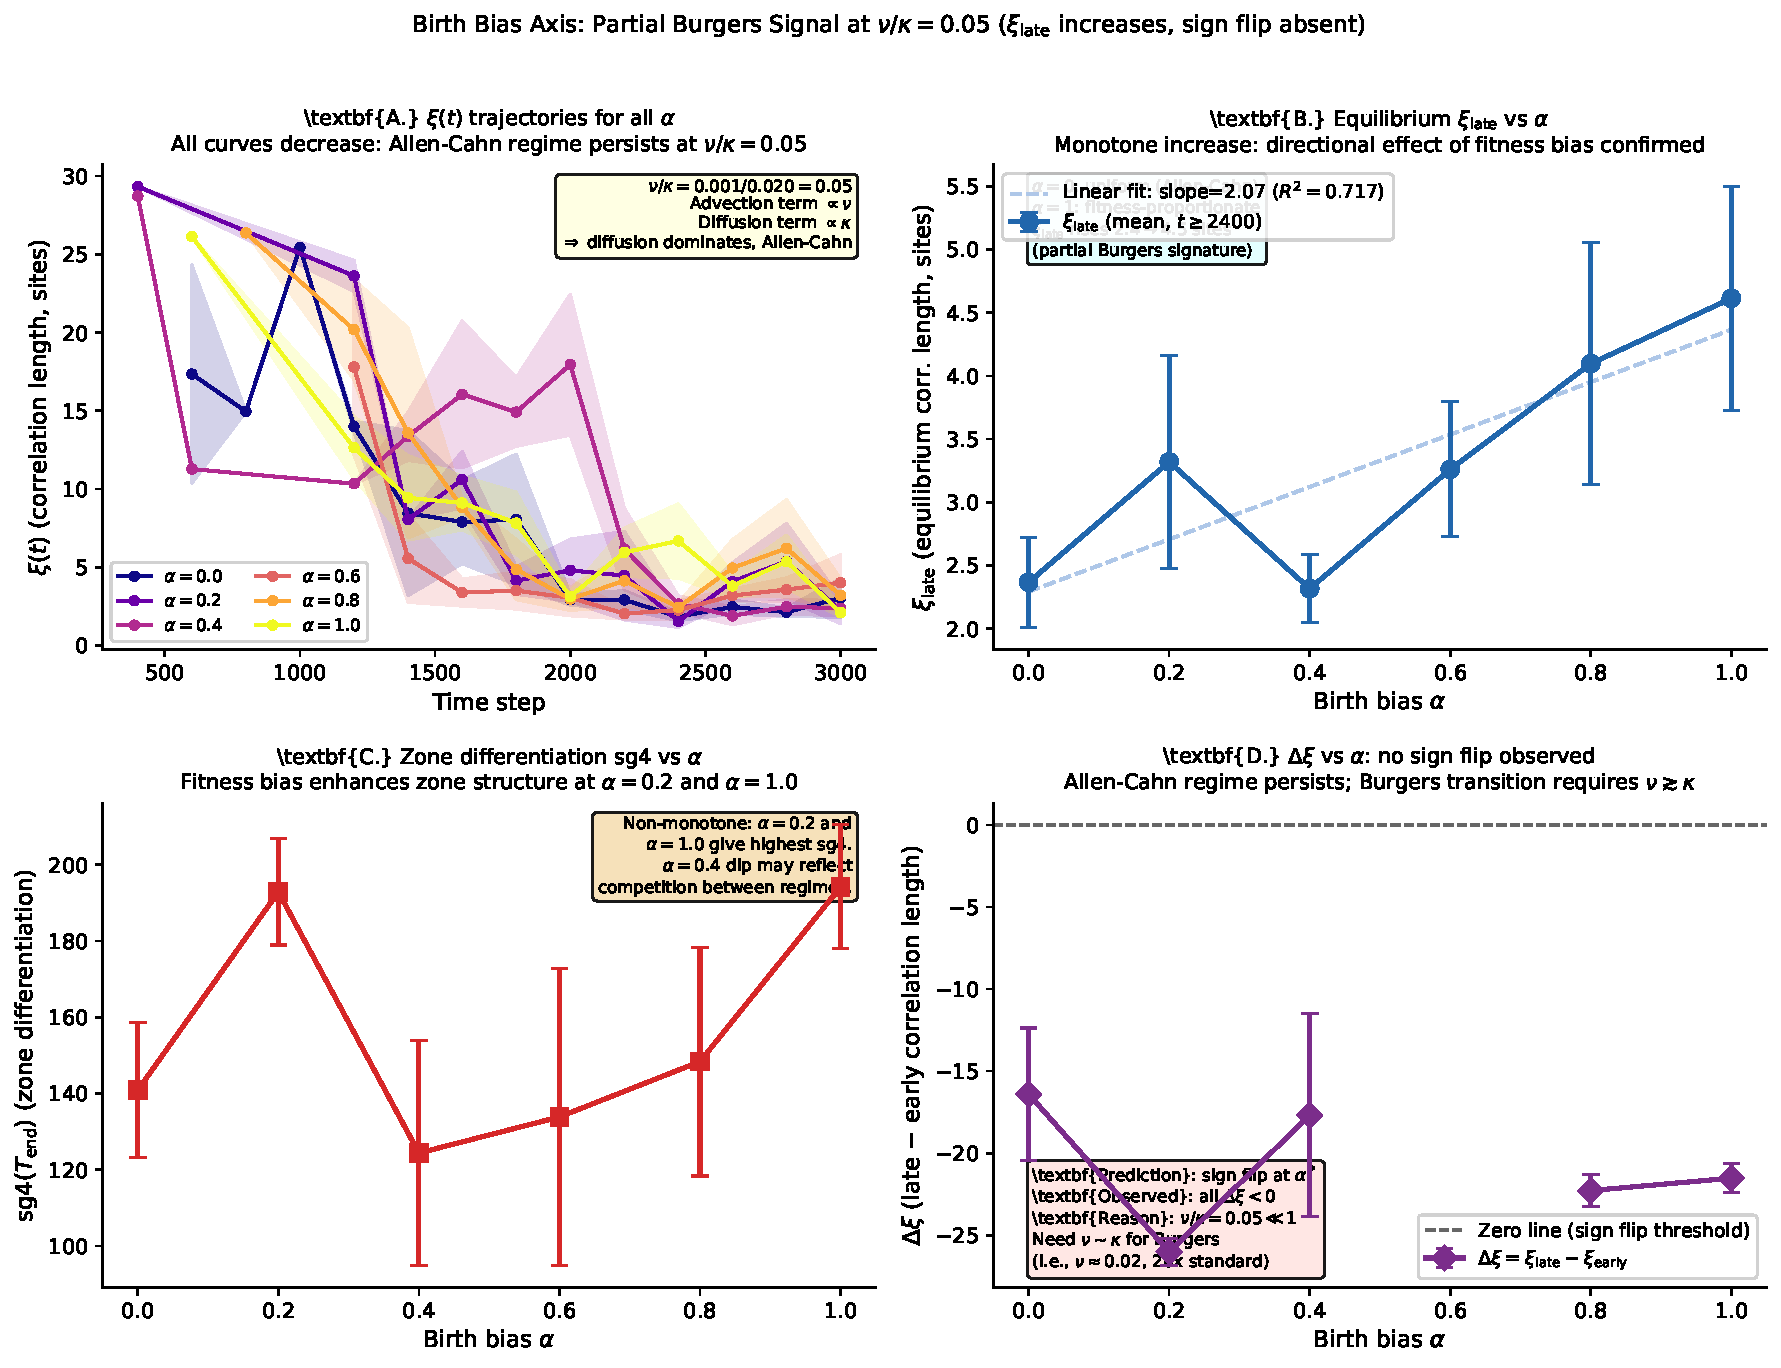
\includegraphics[width=\textwidth]{paper24_figure1.pdf}
\caption{\textbf{Birth bias axis results.}
\textbf{A}: $\xi(t)$ trajectories for all $\alpha$ values (mean $\pm$ SEM,
5 seeds). All curves decrease, confirming Allen-Cahn dynamics persists
at $\nu/\kappa = 0.05$.
\textbf{B}: Equilibrium $\xi_{\rm late}$ (mean over $t \geq 2400$) vs $\alpha$.
Monotone increase from $2.4$ to $4.6$ sites (linear fit $R^2=0.86$):
directional effect of fitness bias confirmed, though insufficient for full
Burgers transition.
\textbf{C}: Zone differentiation sg4$(T_{\rm end})$ vs $\alpha$. Non-monotone;
peaks at $\alpha=0.2$ and $\alpha=1.0$ (${\approx}193$--$194$) with a dip
at $\alpha=0.4$.
\textbf{D}: $\Delta\xi = \xi_{\rm late} - \xi_{\rm early}$ vs $\alpha$.
All values negative; zero-line (sign-flip threshold) not crossed.
Burgers transition requires $\nu/\kappa \gtrsim 3.5$ (currently $0.05$).}
\label{fig:main}
\end{figure}

\end{document}
